\subsection{Gesamtdarstellung des Regelkreises mit PID-gesteuertem DCDC-Konverter}
\label{sec:Gesamtdarstellung_Regelkreis}

Dieser Abschnitt bietet einen umfassenden Überblick über den Regelkreis, der einen PID-Regler, einen Pulsweitenmodulator (PWM) und einen DCDC-Konverter umfasst. Im Mittelpunkt steht die Interaktion dieser Komponenten, die gemeinsam eine konstante Ausgangsspannung gewährleisten. Die Mikroebene der Simulation wird besonders hervorgehoben, um die Auswirkungen der Wechselwirkungen zwischen den einzelnen Elementen auf die Gesamtleistung des Systems zu verdeutlichen.
Abbildung \ref{fig:Regelkreis_Überblick} veranschaulicht den gesamten Regelkreis inklusive des PID-gesteuerten DCDC-Konverters.

\paragraph{Interaktion der Regelkreiskomponenten}
Der Regelungsprozess beginnt mit den vom Actor gelieferten PID-Koeffizienten \( K_p, K_i, \) und \( K_d \), die den PID-Regler ansteuern (siehe Abschnitt \ref{sec:PID-Regler}). Der Regler vergleicht kontinuierlich die aktuelle Spannung mit dem Referenzwert und generiert ein Signal zur Korrektur, das an den PWM weitergeleitet wird.

\paragraph{Funktionsweise des Pulsweitenmodulators (PWM)}
Der PWM-Modulator (Abschnitt \ref{sec:PWM_Grundlagen}) transformiert das Signal des PID-Reglers in eine pulsbreitenmodulierte Form, die den DCDC-Konverter ansteuert. Dieser Konverter sorgt für die Umwandlung der Eingangsspannung in eine stabile Ausgangsspannung. Die Signalverarbeitung im PWM bestimmt die Schaltfrequenz des Transistors im Konverter, um die Last angemessen zu versorgen.

\paragraph{Rolle des DCDC-Konverters}
Der DCDC-Konverter spielt eine zentrale Rolle im Regelkreis, indem er die Energie der Versorgungsspannung in eine nutzbare Ausgangsspannung umwandelt(siehe Abschnitt \ref{sec:DCDC_Konverter}) . Die Arbeitsweise des Konverters ist eng mit den PWM-Signalen verknüpft, welche das Öffnen und Schließen des Transistors steuern. Die PWM regelt die Impulsbreite basierend auf den Steuerbefehlen des PID-Reglers. Diese Impulse beeinflussen das Tastverhältnis und damit die Energiemenge, die durch den Transistor geleitet wird. Die Energie wird in der Induktivität gespeichert und als Strom an die Last abgegeben, wobei die Kapazität als Puffer dient. Änderungen in der Last führen zu Spannungsschwankungen, die der PID-Regler erfasst und ausgleicht, um eine stabile Ausgangsspannung zu gewährleisten.

\paragraph{Integration von Simulation und Realität}
Die Simulation des Regelkreises erfolgte in SystemC, wobei der PID-Regler direkt aus mathematischen Modellen abgeleitet und der PWM sowie der DCDC-Konverter für eine genauere Analyse implementiert wurden. Dies ermöglicht einen Ausgleich zwischen Genauigkeit und Simulationsgeschwindigkeit.


\begin{figure}[htbp]
    \centering
    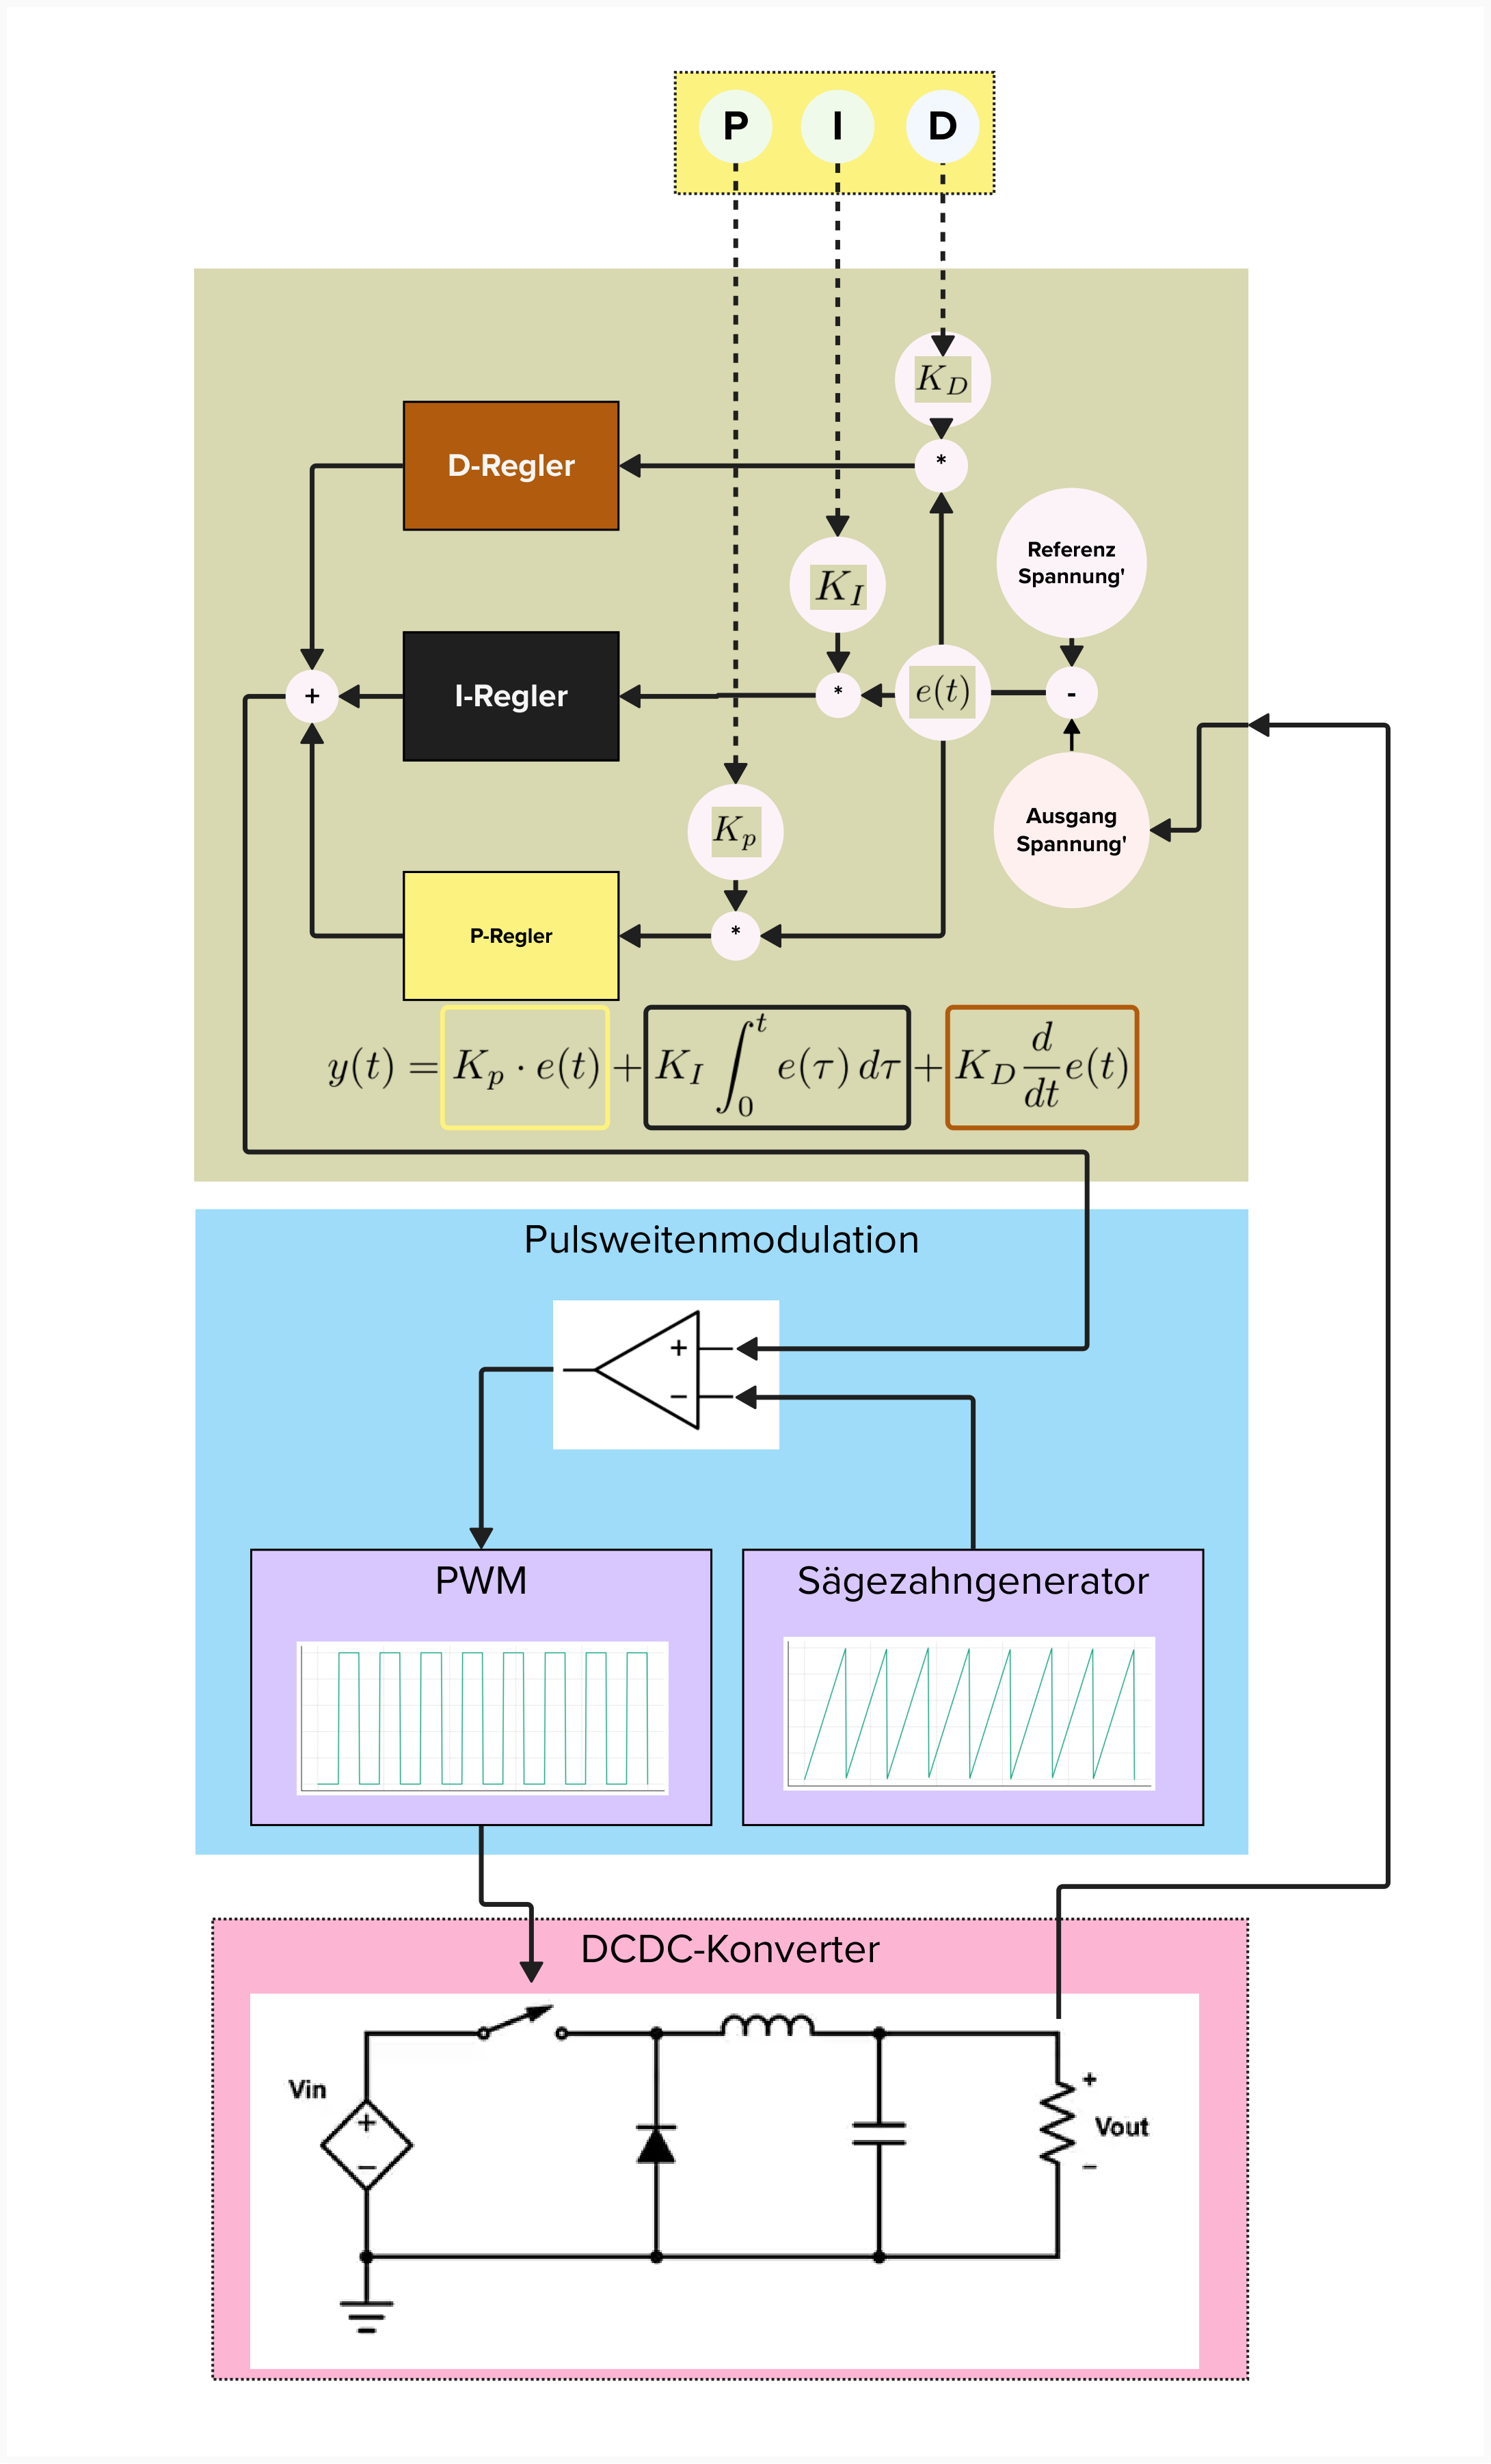
\includegraphics[width=0.99\linewidth]{3Experiment/2Experiment/3PID_Gesteuerter_DCDC_Converter.png}
    \caption{Überblick über den Regelkreis mit dem PID-Regler, PWM und DCDC-Konverter.}
    \label{fig:Regelkreis_Überblick}
\end{figure}
